
\chapter{کارهای پیشین}

در این فصل، به مرور کارهای پیشین و روش‌های مرتبط ترمیم تصویر پرداخته می‌شود. هدف از این مرور، شناسایی نقاط قوت و ضعف روش‌های موجود، بررسی پیشرفت‌های اخیر در حوزه مرتبط، بررسی مجموعه‌داده های ترمیم تصویر و ارائه یک دیدگاه جامع از متدولوژی های مرسوم ترمیم است.

ابتدا به بررسی تاریخچه و پیشرفت روش‌های مرتبط با ترمیم تصاویر پرداخته خواهد شد و دسته‌بندی‌های مختلف این روش‌ها، به همراه مزایا و معایب آن‌ها مورد بحث قرار خواهد گرفت. سپس، مجموعه داده‌های مورد استفاده در این حوزه معرفی شده و معیارهای مورد نظر برای ارزیابی این روش‌ها توضیح داده می‌شوند. در نهایت، الگوریتم‌های کلاسیک و روش‌های مبتنی بر یادگیری عمیق که تاکنون برای ترمیم تصاویر پیشنهاد شده‌اند، بررسی خواهند شد. \textbf{این تحلیل به عنوان مبنایی برای توجیه ضرورت استفاده از معماری \lr{Transformers} در تحقیق حاضر خواهد بود.}



\section{روش های الگوریتمی}

مسئله ترمیم تصویر به قبل‌تر از ظهور روش‌های مبتنی بر یادگیری عمیق بازمی‌گردد. در ابتدا این مسئله به کمک روش‌های الگوریتمی کلاسیک مورد بررسی قرار گرفت. یکی از اولین روش‌های مطرح‌شده در حوزه ترمیم تصاویر، رویکرد مبتنی بر انتشار بود که توسط Bertalmio و همکارانش در سال ۲۰۰۰ معرفی شد \cite{bertalmioImageInpainting2000}. این روش از معادلات دیفرانسیل جزئی \lr{(PDE)} برای گسترش اطلاعات موجود در لبه‌های تصویر به نواحی آسیب‌دیده استفاده می‌کند. ایده اصلی این روش، شبیه‌سازی فرآیند طبیعی انتشار اطلاعات در تصویر است تا ساختارهای محلی به صورت پیوسته بازسازی شوند. با وجود اینکه این روش برای ترمیم نواحی کوچک و حفظ ساختار لبه‌ها عملکرد خوبی دارد، در بازسازی نواحی بزرگ‌تر یا بافت‌های پیچیده به دلیل محدودیت درک محتوای کلی تصویر ناکارآمد است.

در ادامه رویکردهای مبتنی بر انتشار، روش ترمیم تصویر با تغییرات کل \lr{(Total Variation Inpainting)} که توسط Chan و Shen در سال ۲۰۰۱ معرفی شد \cite{chanNontextureInpaintingCurvatureDriven2001}، گامی دیگر در پیشرفت این حوزه بود. این روش بر مبنای به حداقل رساندن یک تابع انرژی طراحی شده است که هدف آن حفظ ساختار لبه‌ها و جلوگیری از ایجاد تاری در نواحی بازسازی‌شده است. مدل تغییرات کل از معادلات دیفرانسیل جزئی برای انتقال اطلاعات لبه‌ها به نواحی آسیب‌دیده استفاده می‌کند و توانایی بالایی در بازسازی ساختارهای ساده دارد. با این حال، مانند روش Bertalmio و همکاران، این رویکرد نیز در بازسازی بافت‌های پیچیده یا نواحی بزرگ با محدودیت‌هایی مواجه است.


دسته دیگری از روش‌های کلاسیک، روش‌های مبتنی بر وصله \lr{(Patch-Based Methods)} بودند که از آماره‌های غیرمحلی برای بازسازی تصویر استفاده می‌کردند. در این روش‌ها، نواحی سالم تصویر به عنوان بانک وصله‌ها در نظر گرفته می‌شدند و بهترین تطابق برای پر کردن نواحی آسیب‌دیده از میان این وصله‌ها انتخاب می‌شد.

به‌عنوان مثال در یکی از برجسته ترین روش های غیرمبتنی بر یادگیری، بارنز و همکاران در \cite{barnesPatchMatchRandomizedCorrespondence2009} با معرفی PatchMatch ابزارهای تعاملی ویرایش تصویر را با استفاده از یک الگوریتم تصادفی جدید ارائه داده‌اند که امکان یافتن بسیار سریع تطابق‌های تقریبی نزدیک‌ترین همسایه بین قطعات تصویر را فراهم می‌کند. الگوریتم ارائه‌شده توسط آن‌ها بهبودهای قابل‌توجهی در عملکرد نسبت به روش‌های پیشین (۲۰ تا ۱۰۰ برابر سریع‌تر) ارائه می‌دهد و استفاده از آن را در ابزارهای تعاملی ممکن می‌سازد. بینش‌های کلیدی این الگوریتم شامل یافتن برخی تطابق‌های مناسب از طریق نمونه‌گیری تصادفی و استفاده از هم‌بستگی طبیعی در تصاویر برای انتشار سریع این تطابق‌ها به نواحی مجاور است.

با وجود این که این رویکردها توانستند نتایج بهتری در بازسازی جزئیات ارائه دهند، اما به دلیل تکیه بر ویژگی‌های محلی و وابستگی به مشابهت بافتی، در مواجهه با تصاویر پیچیده و متنوع محدودیت‌های زیادی داشتند و اکثرا مفروضات عمیقی در مورد تصاویر هدفشان داشتند. یکی از این مفروضات، فرض رنک پایین بودن تصاویر است. این فرض بر این ایده استوار است که داده‌های تصویری در بسیاری از کاربردها، به‌ویژه در تصاویر طبیعی، به صورت ذاتی دارای ساختار رنک پایین هستند. به این معنا که اطلاعات موجود در یک تصویر را می‌توان در یک فضای برداری با ابعاد بسیار کمتر نسبت به فضای اصلی بازنمایی کرد. روش‌های مبتنی بر این فرض، مانند تجزیه مقدار منفرد \lr{(SVD)}
\cite{yaghmaeeImprovingImageInpainting2020}
 و فشرده‌سازی رنک پایین، در بسیاری از مسائل پردازش تصویر نظیر ترمیم تصویر، کاهش نویز و فشرده‌سازی داده به کار گرفته شدند. با این حال، این الگوریتم‌های کلاسیک اغلب در شرایط پیچیده‌تر مانند تصاویر با ساختار غیرخطی، نواحی هدف ترمیم بسیار بزرگ، نواحی بافت‌های پیچیده، یا تصاویر آسیب‌دیده با نویز بالا عملکرد ضعیفی داشتند.

این محدودیت‌ها ناشی از این واقعیت است که تصاویر واقعی معمولاً از روابط غیرخطی پیچیده و وابستگی‌های بلندمدت میان پیکسل‌ها پیروی می‌کنند که فرض رنک پایین قادر به مدل‌سازی آن‌ها نیست. علاوه بر این، این روش‌ها اغلب فرض می‌کنند که اطلاعات کلیدی تصویر به صورت یکنواخت توزیع شده است، در حالی که در واقعیت، اطلاعات تصاویر در نواحی مختلف دارای توزیع‌های بسیار متفاوتی است.


\section{روش‌های مبتنی بر یادگیری عمیق}

با ظهور یادگیری عمیق و توانایی آن در استخراج ویژگی‌های پیچیده از داده‌های تصویری، پژوهش‌ها در زمینه ترمیم تصاویر به سمت استفاده از مدل‌های مبتنی بر شبکه‌های عصبی سوق یافت. این روش‌ها با استفاده از مجموعه داده‌های بزرگ و متنوع، قادر به یادگیری الگوهای پیچیده و بازسازی دقیق‌تر نواحی آسیب‌دیده شدند. برخلاف روش‌های الگوریتمی که عمدتاً بر اصول ریاضی و آماری استوار بودند، روش‌های مبتنی بر یادگیری امکان درک مفاهیم سطح بالا و روابط جهانی در تصویر را فراهم کردند و موفق شدند ترمیم هایی با  ماسک های بزرگ‌تر انجام دهند، چرا که این امر گاها نیازمند ساخت ساختار های کاملا جدید در تصویر (مانند ساختار چهره، طبیعت و ...) بود.

در مقایسه با روش‌های سنتی، روش‌های مبتنی بر یادگیری در ترمیم تصاویر موفقیت چشمگیری کسب کرده‌اند، به‌ویژه زمانی که صحبت از تولید محتوای جدید و همخوان با زمینه برای نواحی بزرگ حذف‌شده باشد.

\section{مجموعه‌داده‌های ترمیم تصویر}

یکی از عوامل کلیدی در موفقیت مدل‌های یادگیری عمیق در پردازش تصویر، وجود مجموعه‌داده‌های بزرگ و متنوع است که امکان آموزش مدل‌ها در سناریوهای گوناگون را فراهم می‌سازد. مجموعه‌داده‌های مختلف برای کاربردهای خاص طراحی شده‌اند و هر یک ویژگی‌های منحصربه‌فردی دارند. در ادامه، به معرفی برخی از مجموعه‌داده‌های شناخته‌شده مانند \lr{CelebA-HQ}، \lr{Places}، و چندین مجموعه‌داده دیگر پرداخته می‌شود.


مجموعه‌داده \textbf{CelebA-HQ} یکی از معروف‌ترین مجموعه‌داده‌ها برای تحلیل چهره است. این مجموعه‌داده‌ی علامت‌گذاری نشده، شامل تصاویری با وضوح بالا از چهره انسان است که ویژگی‌هایی مانند موقعیت، حالت، و روشنایی مختلف را پوشش می‌دهد. CelebA-HQ به‌طور گسترده در زمینه‌هایی مانند بازسازی تصویر، تغییر چهره، و شناسایی چهره استفاده شده است. ویژگی برجسته این مجموعه‌داده، کیفیت بالای تصاویر و پوشش گسترده از حالات و ویژگی‌های مختلف چهره است که آن را به انتخابی محبوب برای مدل‌های یادگیری عمیق تبدیل کرده است.

\begin{figure}
	\centering
	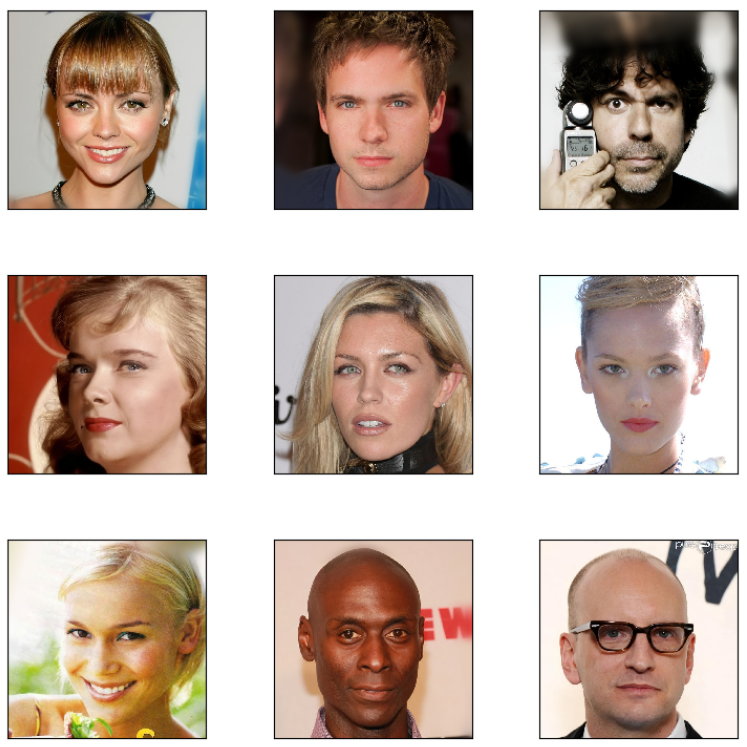
\includegraphics[width=0.7\linewidth]{celebahq1}
	\caption{نمونه تصاویر از مجموعه‌داده Celeb-A-HQ. تمرکز این دیتاست بر روی فیچر های چهره است.}
	\label{fig:celebahq1}
\end{figure}

مجموعه‌داده \textbf{Places} برای تحلیل صحنه‌ها و شناخت محیط‌ها طراحی شده است. این مجموعه‌داده‌ی علامت‌گذاری شده، شامل میلیون‌ها تصویر از محیط‌های مختلف مانند مناظر طبیعی، محیط‌های شهری، و فضاهای داخلی است. مجموعه Places برای کاربردهایی مانند تشخیص صحنه، طبقه‌بندی محیط، و تولید تصاویر صحنه استفاده می‌شود. یکی از ویژگی‌های کلیدی این مجموعه‌داده، تنوع بالا در دسته‌بندی‌های محیطی است که امکان آموزش مدل‌هایی با درک عمیق‌تر از صحنه‌های مختلف را فراهم می‌کند.

\begin{figure}
	\centering
	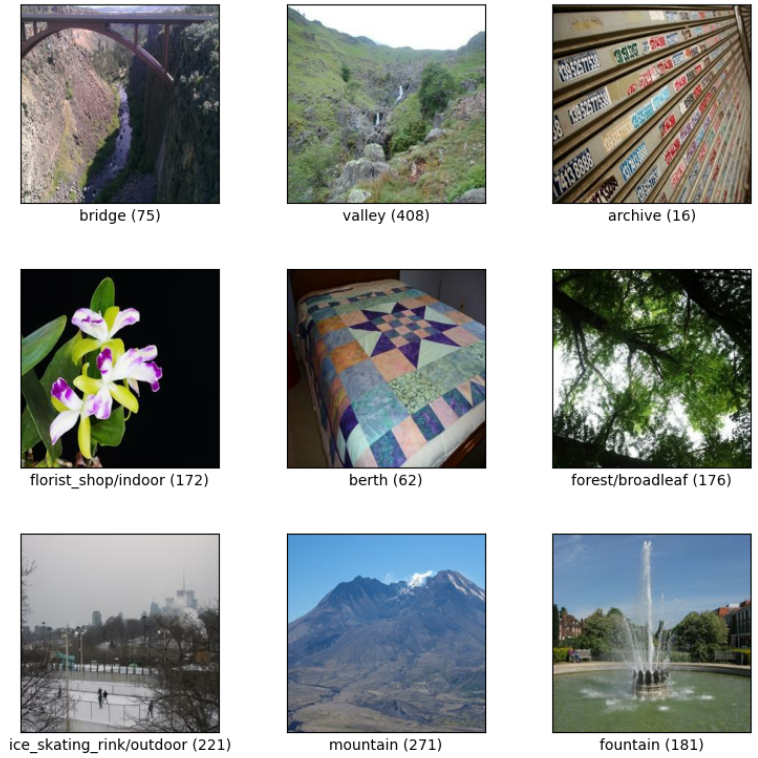
\includegraphics[width=0.7\linewidth]{places1}
	\caption{نمونه تصاویر از مجموعه‌داده Places به همراه یک کلمه برای توصیف هر تصویر و نام هر فایل در داخل پرانتز}
	\label{fig:places1}
\end{figure}


مجموعه‌داده \textbf{ImageNet} یکی از جامع‌ترین مجموعه‌داده‌های موجود در حوزه یادگیری عمیق است که با بیش از ۱۴ میلیون تصویر در ۱۰۰۰ طبقه‌بندی مختلف تأثیر شگرفی بر پیشرفت شبکه‌های عصبی داشته است. ImageNet علاوه بر کاربردهای عمومی مانند طبقه‌بندی تصویر، به‌عنوان یک معیار استاندارد برای ارزیابی عملکرد مدل‌های یادگیری عمیق استفاده می‌شود. موفقیت‌های اولیه شبکه‌های عصبی کانولوشنی (CNN) مانند AlexNet و ResNet تا حد زیادی مرهون این مجموعه‌داده بزرگ و متنوع بوده‌اند.



%یکی دیگر از مجموعه‌داده‌های مهم، \textbf{MS-COCO} است که برای وظایف پیشرفته‌تری مانند تشخیص اشیا، بخش‌بندی تصویر، و توصیف تصویر طراحی شده است. این مجموعه‌داده شامل تصاویری است که حاوی چندین شیء از دسته‌بندی‌های مختلف هستند، و هر تصویر دارای برچسب‌های متنی دقیق و اطلاعات مربوط به موقعیت اشیاء است. MS-COCO به‌طور گسترده در مدل‌هایی که نیازمند درک پیچیده‌تر تصویر هستند، مانند مدل‌های تولید متن از تصویر
%\LTRfootnote{Image Captioning}
%یا سیستم‌های تشخیص چند‌شیء، استفاده می‌شود.
مجموعه داده
\lr{DTD (Describable Textures Dataset)}
یک مجموعه داده شامل $5640$ تصویر واقعی از بافت‌های مختلف است که با یک یا چند صفت توصیفی از یک واژگان ۴۷ کلمه‌ای در زبان انگلیسی برچسب‌گذاری شده‌اند. این مجموعه داده به‌طور خاص برای مطالعه و تحلیل بافت‌های قابل توصیف طراحی شده است و شامل نمونه‌هایی از بافت‌های طبیعی و مصنوعی است. 

از ویژگی‌های قابل توجه \lr{DTD} می‌توان به تنوع گسترده تصاویر و برچسب‌های توصیفی دقیق اشاره کرد که آن را به یک منبع ارزشمند در کاربردهایی نظیر دسته‌بندی بافت‌ها، تشخیص الگو و آموزش مدل‌های یادگیری عمیق تبدیل کرده است. این مجموعه داده برای ارزیابی مدل‌های بینایی کامپیوتر که نیاز به درک ویژگی‌های بصری بافت‌ها دارند، به‌ویژه در مسائل مرتبط با توصیف و دسته‌بندی، بسیار مناسب است.

\begin{figure}
	\centering
	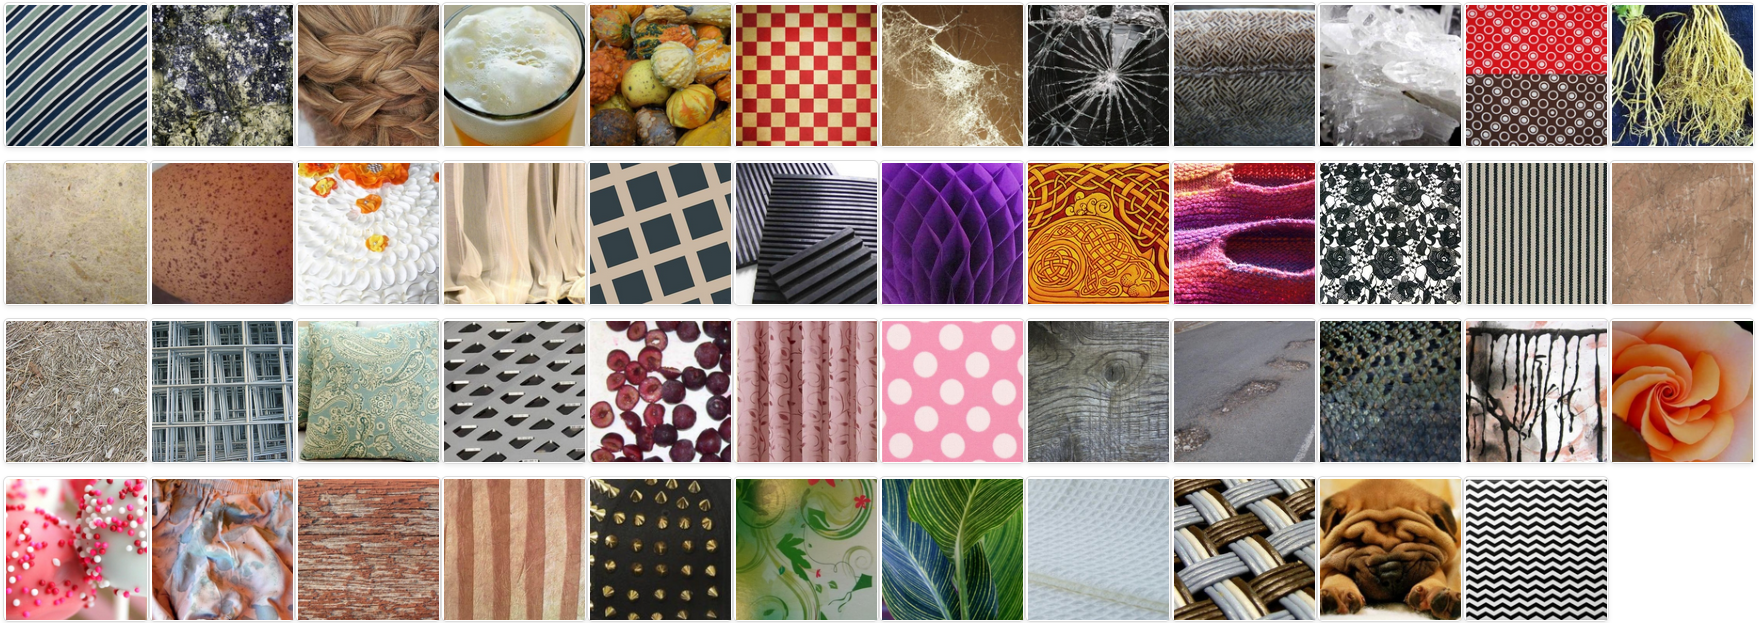
\includegraphics[width=0.7\linewidth]{dtd1}
	\caption{نمونه تصاویر مجموعه‌داده DTD}
	\label{fig:dtd1}
\end{figure}



\begin{table}
	\centering
	\label{tab:datasets_summary}
	\begin{tabular}{|l|c|c|l|}
		\hline
		\textbf{نام مجموعه داده} & \textbf{برچسب‌دار (بله/خیر)} & \textbf{تعداد تصاویر} & \textbf{ویژگی} \\ \hline
		\lr{Places2} \cite{zhouPlacesImageDatabase2016} & بله & $>10,000,000$ & محیط‌ها \\ \hline
		\lr{CelebA} \cite{liuDeepLearningFace2015} & بله & $200,000$ & چهره \\ \hline
		\lr{CelebHQ} \cite{karrasProgressiveGrowingGANs2018} & بله & $30,000$ & چهره با کیفیت \\ \hline
		\lr{DTD} \cite{cimpoiDescribingTexturesWild2013} & بله & $5,640$ & بافت \\ \hline
		\lr{ImageNet} \cite{russakovskyImageNetLargeScale2015} & بله &  $>14,000,000$
		\tablefootnote{این مجموعه‌داده هر سال در حال بروزرسانی و افزوده شدن است. آمار ذکر شده آخرین آمار تا ژانویه ۲۰۲۵ است.}
		 & اشیاء \\ \hline
	\end{tabular}
	\caption{خلاصه‌ای از مجموعه داده‌های معروف}
\end{table}


\begin{figure}
	\centering
	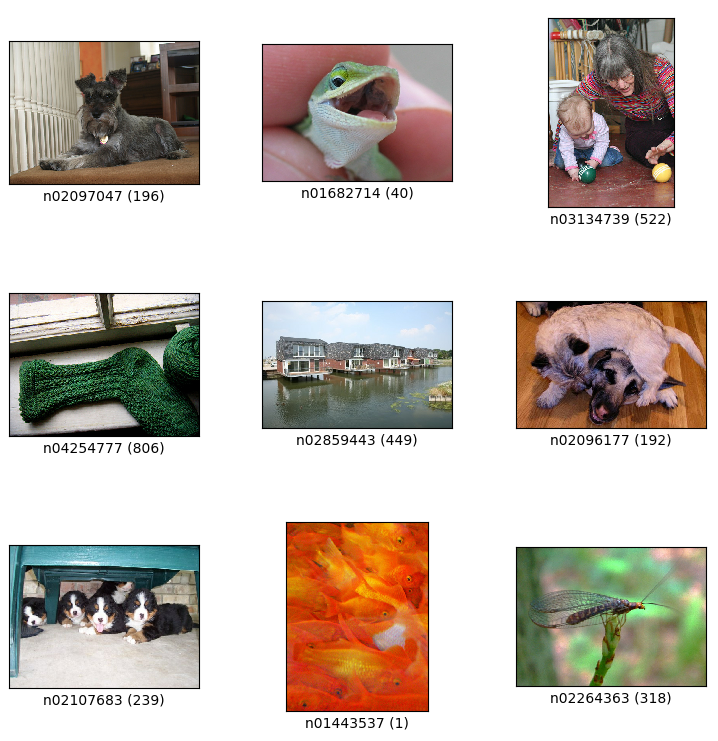
\includegraphics[width=0.7\linewidth]{imagenet2012-1}
	\caption{نمونه تصاویر از مجموعه‌داده
		ImageNet
		نسخه سال ۲۰۱۲ به همراه یک کلمه برای توصیف هر تصویر و نام هر فایل در داخل پرانتز}
	\label{fig:imagenet2012-1}
\end{figure}


Pathak
و همکاران در \cite{pathakContextEncodersFeature2016}
یک الگوریتم یادگیری ویژگی‌های بصری بدون نظارت \LTRfootnote{Unsupervised} ارائه داده‌اند که بر اساس پیش‌بینی پیکسل مبتنی بر زمینه هدایت می‌شود. به‌طور مشابه با خودرمزگذارها
\LTRfootnote{Autoencoders}
، آن‌ها \lr{Context Encoders} را پیشنهاد کرده‌اند – یک شبکه عصبی کانولوشنی که برای تولید محتوای یک ناحیه دلخواه از تصویر، با توجه به محیط اطراف آن آموزش داده شده است. برای موفقیت در این وظیفه، \lr{Context Encoders} باید هم محتوای کل تصویر را درک کنند و هم فرضیه‌ای معقول برای قسمت‌های حذف‌شده ارائه دهند.  

آن‌ها در آموزش \lr{Context Encoders}،‌ از دو رویکرد استفاده کرده‌اند: یکی اتکای صرف به تابع هزینه بازسازی پیکسل-محور استاندارد بر اساس نرم دوم (\lr{L2 Loss})، و دیگری ترکیب بازسازی با یک تابع هزینه رقابتی (\lr{Adversarial Loss}) پیشنهاد شده در شبکه های GAN
\cite{goodfellowGenerativeAdversarialNetworks2014}.
نتایج نشان داده است که رویکرد دوم خروجی‌هایی با وضوح بالاتر تولید می‌کند، زیرا بهتر می‌تواند حالت‌های چندگانه در خروجی را مدیریت کند.  

\begin{figure}
	\centering
	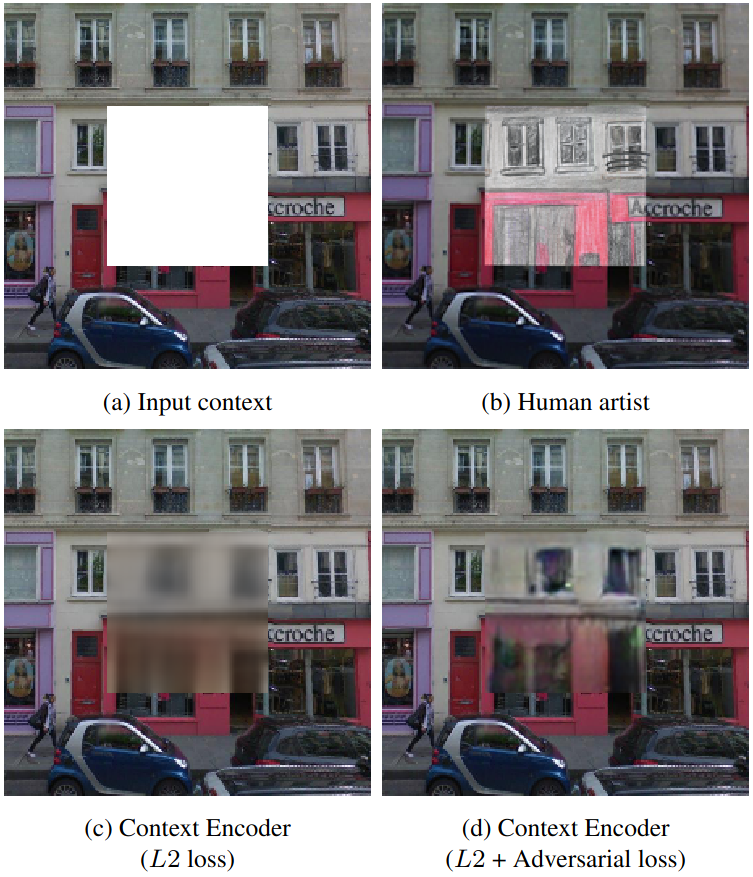
\includegraphics[width=0.7\linewidth]{figs/contextencodersLossComparison}
	\caption{مقایسه کیفی  استفاده از تابع هزینه نرم  ۲ در مقابل استفاده از یک تابع هزینه رقابتی در خروجی های تولید شده. 
		(a) عکس ورودی با یک قسمت از دست رفته 
		(b) یک انسان هنرمند مشکلی در ترمیم این تصویر ندارد 
		(c)
ترمیم خودکار تصویر با استفاده از \lr{Context Encoders} که توسط تابع هزینه بازسازی بر اساس نرم ۲ آموزش داده شده است.
	(d)
ترمیم خودکار تصویر با استفاده از \lr{Context Encoders} که توسط تابع هزینه رقابتی آموزش داده شده است.
}
	\label{fig:contextencoderslosscomparison}
\end{figure}



آن‌ها دریافتند  \lr{Context Encoders} بازنمایی ای یاد می‌گیرند که نه‌تنها ظاهر، بلکه معنای ساختارهای بصری را نیز در بر می‌گیرد. اثربخشی این ویژگی‌های یادگرفته‌شده به‌طور کمّی برای پیش‌آموزش شبکه‌های عصبی کانولوشنی (CNN) در وظایف طبقه‌بندی، تشخیص و قطعه‌بندی نشان داده شده است. علاوه بر این، \lr{Context Encoders} می‌توانند برای وظایف ترمیم معنایی تصاویر \lr{(Semantic Inpainting)} مورد استفاده قرار گیرند، چه به‌صورت مستقل و چه به‌عنوان نقطه شروع برای روش‌های غیرپارامتری.
\begin{figure}
	\centering
	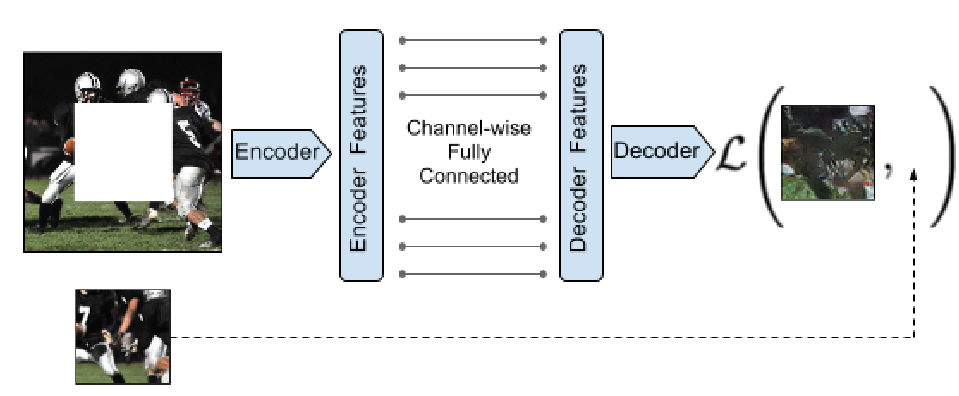
\includegraphics[width=0.7\linewidth]{figs/contextencodersArchitecture}
	\caption[معماری کلی Context Encoders]{
	تصویر زمینه از طریق بخش رمزگذار عبور داده می‌شود تا ویژگی‌هایی استخراج شوند که از طریق یک لایه کاملاً متصل کانال‌محور به رمزگشا متصل می‌شوند. سپس، رمزگشا نواحی حذف‌شده تصویر را تولید می‌کند.}
	\label{fig:contextencodersarchitecture}
\end{figure}

به دنبال این روش، روش های بسیاری بر پایه GAN ابداع شدند. 
\cite{caoLearningSketchTensor2021}
\cite{guoImageInpaintingConditional2024}
\cite{liRecurrentFeatureReasoning2020}
\cite{nazeriEdgeConnectGenerativeImage2019}
\cite{pengGeneratingDiverseStructure2021}

به عنوان مثال


!TODO HERE

\section{روش های ارزیابی}

\subsection{معیار PSNR}
معیار PSNR (نسبت سیگنال به نویز پیک) رابطه‌ای است بین انرژی حداکثری یک سیگنال و نویزی که بر دقت نمایش آن تأثیر می‌گذارد. در زمینه ترمیم تصویر (inpainting)، این معیار به رابطه‌ای بین تصویر اصلی (Ground Truth) و تصویر ترمیم‌شده اشاره دارد. هرچه مقدار PSNR بالاتر باشد، کیفیت تصویر ترمیم‌شده بهتر خواهد بود.

برای محاسبه PSNR یک تصویر آزمایشی (g) با استفاده از تصویر مرجع (f)، ابتدا نیاز است که میانگین مربعات خطا (MSE) محاسبه شود. این مقدار از طریق معادله زیر به دست می‌آید:

\[
MSE = \frac{1}{N} \sum_{i=1}^{N} (f_i - g_i)^2
\]

که در آن $f_i$ و $g_i$ به ترتیب مقدار پیکسل‌های تصویر مرجع و تصویر آزمایشی هستند و $N$ تعداد کل پیکسل‌ها می‌باشد. پس از محاسبه MSE، مقدار PSNR به‌صورت زیر محاسبه می‌شود:

\begin{equation}
PSNR = 10 \cdot \log_{10}\left(\frac{MAX^2}{MSE}\right)
\end{equation}

در اینجا $MAX$ مقدار حداکثری شدت پیکسل‌ها در تصویر است (برای تصاویر 8 بیتی معمولاً برابر با 255 است). PSNR معیاری برای ارزیابی کیفیت تصویر است که هرچه مقدار آن بیشتر باشد، به معنای کیفیت بالاتر تصویر ترمیم‌شده است.

\subsection{معیار SSIM}

SSIM (شاخص مشابهت ساختاری) یک تکنیک برای اندازه‌گیری مشابهت بین دو تصویر است. این روش یک تصویر با کیفیت کامل را با تصویر دیگری مقایسه می‌کند. در زمینه ترمیم تصویر (inpainting)، SSIM تصویر اصلی را با تصویر ترمیم‌شده مقایسه می‌کند. این معیار توانایی مدل در حفظ ساختار و ویژگی‌های تصویر اصلی را اندازه‌گیری می‌کند.

مناطق با مقادیر کوچک SSIM محلی نشان‌دهنده مناطقی هستند که تصویر ترمیم‌شده از تصویر مرجع تفاوت دارد. این مقادیر پایین به‌ویژه در نواحی آسیب‌دیده یا ترمیم‌شده مشاهده می‌شوند که در آن‌ها مدل نتوانسته است جزئیات تصویر اصلی را به‌خوبی بازسازی کند. برعکس، مقادیر بزرگ SSIM در نواحی یکنواخت تصویر مرجع مشاهده می‌شود، جایی که تصویر ترمیم‌شده مشابه تصویر اصلی است و تفاوت‌های کمی بین آن‌ها وجود دارد.

فرمول کلی SSIM به صورت زیر است:
$$
SSIM(f, g) = l(f, g) \cdot c(f, g) \cdot s(f, g)
$$

که در آن $l(f, g)$، $c(f, g)$ و $s(f, g)$ به ترتیب مولفه‌های روشنایی (luminance)، کنتراست (contrast) و ساختار (structure) هستند. این مولفه‌ها به شرح زیر تعریف می‌شوند:

\textbf{مولفه روشنایی}%
\LTRfootnote{Luminance}
: این مولفه تفاوت میانگین شدت روشنایی بین دو تصویر را اندازه‌گیری می‌کند. اگر میانگین شدت روشنایی تصویر مرجع ($\mu_f$) و تصویر ترمیم‌شده ($\mu_g$) نزدیک به هم باشند، مقدار $l(f, g)$ به 1 نزدیک می‌شود، که نشان‌دهنده شباهت بالا در روشنایی کلی است.
$$
l(f, g) = \frac{2\mu_f \mu_g + C_1}{\mu_f^2 + \mu_g^2 + C_1}
$$
که در آن $\mu_f$ و $\mu_g$ میانگین پیکسل‌های تصویر مرجع و تصویر ترمیم‌شده هستند، و $C_1$ یک مقدار ثابت کوچک برای جلوگیری از تقسیم بر صفر است.

\textbf{مولفه کنتراست}%
\LTRfootnote{Contrast}
:    این مولفه تغییرپذیری شدت پیکسل‌ها را در هر تصویر مقایسه می‌کند. اگر انحراف معیار ($\sigma_f$ و $\sigma_g$) دو تصویر مشابه باشند، مقدار $c(f, g)$ به 1 نزدیک می‌شود، که نشان می‌دهد کنتراست (تفاوت بین روشن‌ترین و تاریک‌ترین نواحی) در هر دو تصویر مشابه است.
$$
c(f, g) = \frac{2\sigma_f \sigma_g + C_2}{\sigma_f^2 + \sigma_g^2 + C_2}
$$
که در آن $\sigma_f$ و $\sigma_g$ انحراف معیار پیکسل‌های تصویر مرجع و تصویر ترمیم‌شده هستند، و $C_2$ مقدار ثابتی مشابه $C_1$ است.

\textbf{مولفه ساختار}
: این مولفه شباهت ساختاری بین دو تصویر را ارزیابی می‌کند. ساختار به رابطه بین پیکسل‌ها و همبستگی آن‌ها با یکدیگر اشاره دارد. اگر تصاویر مرجع و ترمیم‌شده دارای الگوهای ساختاری مشابه باشند (مثلاً در لبه‌ها و جزئیات)، مقدار $s(f, g)$ به 1 نزدیک خواهد بود.
$$
s(f, g) = \frac{\sigma_{fg} + C_3}{\sigma_f \sigma_g + C_3}
$$
که در آن $\sigma_{fg}$ همبستگی میان تصویر مرجع و تصویر ترمیم‌شده است، و $C_3$ مقدار ثابت دیگری برای جلوگیری از تقسیم بر صفر است.

ترکیب این سه مؤلفه از طریق ضرب آن‌ها تضمین می‌کند که SSIM تنها در صورتی مقدار بالایی خواهد داشت که تصاویر از نظر روشنایی، کنتراست و ساختار به یکدیگر بسیار شبیه باشند.

SSIM
 به طور کلی به‌عنوان یک معیار بهتر از PSNR در ارزیابی کیفیت بصری تصویر شناخته می‌شود، چرا که SSIM قادر است ویژگی‌های بصری و ساختاری تصویر را با دقت بیشتری مدل‌سازی کند و علاوه بر اندازه‌گیری خطاهای نقطه‌ای، به ویژگی‌های ساختاری تصویر نیز توجه می‌کند و می‌تواند اطلاعات بیشتری در مورد شباهت‌های بصری بین دو تصویر ارائه دهد. این ویژگی به‌ویژه در ارزیابی تصاویر ترمیم‌شده که ممکن است خطاهای محلی داشته باشند، مفید است.






این استراتژی‌ها همگی به دنبال این هستند که روش‌های مؤثری برای استخراج اطلاعات معتبر از نواحی شناخته‌شده تصویر به منظور پر کردن حفره‌ها پیدا کنند. هدف اصلی این رویکردها، بهره‌برداری بهینه از اطلاعات زمینه‌ای و استفاده از آن‌ها برای بازسازی نواحی گمشده است. با این حال، این روش‌ها هنوز با مشکلی اساسی روبرو هستند: از دست رفتن اطلاعاتی که در فرآیند نمونه‌برداری رو به پایین (\lr{Downsampling}) در شبکه‌های کانولوشنی رخ می‌دهد.  

این فرآیند نمونه‌برداری که برای کاهش ابعاد داده و افزایش بازده محاسباتی در شبکه‌های عصبی مورد استفاده قرار می‌گیرد، اغلب منجر به حذف جزئیات ظریف و اطلاعات ضروری می‌شود که می‌توانند برای بازسازی دقیق‌تر و واقعی‌تر مناطق گمشده نقش کلیدی ایفا کنند. بنابراین، یکی از چالش‌های مهم این است که چگونه می‌توان ضمن بهره‌گیری از مزایای نمونه‌برداری رو به پایین، تأثیرات منفی آن را کاهش داد و اطلاعات از دست رفته را تا حد ممکن حفظ کرد.